%- - - - - - - - - - - - - - - - - - - - - - - - - - - - - - - - - SLIDE -
\begin{frame}
 \frametitle{Tópicos Avançados em Programação}
 \begin{block}{Metodologia}
  \begin{itemize}
   \item Apresentação de material em início da aula.
   \item Resolução de problema(s) durante o resto da aula.
   \item Resolução de problema(s) em trabalhos fora de aula (dever de casa).
   \item Divisão da disciplina:
    \begin{itemize}
     \item apresentação de recursos de linguagem.% [Vagner]
     \item apresentação de algumas (classes de) soluções clássicas.% [Humberto/Vagner]
     \item estudo e apresentação de soluções clássicas.% [Alunos]
    \end{itemize}
   \item O nível dos problemas deverá ir crescendo.
%    \item Modelo: \url{http://www.cs.sunysb.edu/~skiena/392/index.html}
  \end{itemize}
 \end{block}
\end{frame}
%- - - - - - - - - - - - - - - - - - - - - - - - - - - - - - - - - SLIDE -
\begin{frame}
 \frametitle{Tópicos Avançados em Programação}
 \begin{block}{Avaliação}
  \begin{itemize}
   \item Nota 1:
    \begin{description}[40\%]
     \item [30\%] Dever de casa.
     \item [30\%] Problemas resolvidos durante as aulas.
     \item [40\%] Desempenho durante a competição de avaliação.
    \end{description}
   \item Nota 2:
    \begin{description}[40\%]
     \item [30\%] Dever de casa.
     \item [30\%] Problemas resolvidos durante as aulas.
     \item [40\%] Desempenho durante a competição de avaliação.
    \end{description}
   \item Nota 3:
    \begin{description}[40\%]
     \item [30\%] Dever de casa.
     \item [30\%] Problemas resolvidos durante as aulas.
     \item [40\%] Desempenho durante a competição de avaliação.
    \end{description}
  \end{itemize}
 \end{block}
\end{frame}
%- - - - - - - - - - - - - - - - - - - - - - - - - - - - - - - - - SLIDE -
\begin{frame}
 \frametitle{Tópicos Avançados em Programação}
 \begin{block}{Avaliação}
  \begin{itemize}
   \item Pontos extras serão atribuídos às atividades extras.
   \item Prazos:
    \begin{itemize}
     \item O dever de casa deve ser entregue até a aula seguinte.
     \item Deveres de casa atrasados não serão aceitos.
    \end{itemize}
   \item Expectativa (dever de casa):
    \begin{itemize}
     \item Um problema por semana: nota entre 6 e 8.
     \item Dois problemas por semana: acima de 8.
    \end{itemize}
  \end{itemize}
 \end{block}
\end{frame}
%- - - - - - - - - - - - - - - - - - - - - - - - - - - - - - - - - SLIDE -
\begin{frame}
 \frametitle{Tópicos Avançados em Programação}
 \begin{block}{Bibliografia: livro texto}
  \centering
  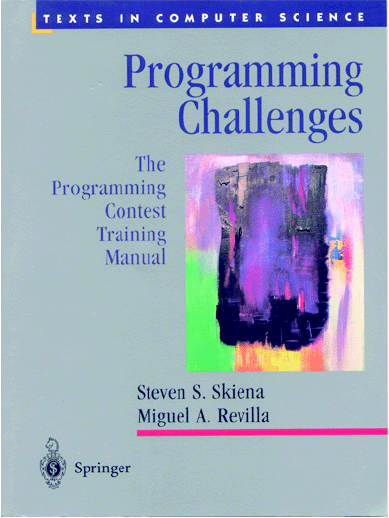
\includegraphics[height=.5\textheight]{figuras/prog-chall-book}
 \end{block}
 \begin{block}{}
  Art of Programming Contest. 2nd Edition. Ahmed Shamsul Arefin. ISBN 984-32-3382-4.
 \end{block}
\end{frame}
%- - - - - - - - - - - - - - - - - - - - - - - - - - - - - - - - - SLIDE -
\begin{frame}
 \frametitle{Tópicos Avançados em Programação}
 \begin{block}{Bibliografia: outros livros}
  \centering
  \includegraphics[width=.9\textwidth]{figuras/prog-books}
 \end{block}
\end{frame}
%- - - - - - - - - - - - - - - - - - - - - - - - - - - - - - - - - SLIDE -
